\documentclass[12pt]{article}
\usepackage[danish]{babel}
\usepackage{amsfonts, amssymb, mathtools, amsthm, amsmath}
\usepackage{graphicx, pgfplots}
\usepackage{url}
\usepackage[dvipsnames]{xcolor}
\usepackage{sagetex}
\usepackage{lastpage}

%loaded last
\usepackage[hidelinks]{hyperref}

\usepackage{siunitx}
  \sisetup{exponent-product = \cdot,
    output-decimal-marker = {,}}

%Giles Castelles incfig
\usepackage{import}
\usepackage{xifthen}
\usepackage{pdfpages}
\usepackage{transparent}

\newcommand{\incfig}[2][1]{%
  \def\svgwidth{#1\columnwidth}
  \import{../figures/}{#2.pdf_tex}
}

\setlength{\parindent}{0in}
\setlength{\oddsidemargin}{0in}
\setlength{\textwidth}{6.5in}
\setlength{\textheight}{8.8in}
\setlength{\topmargin}{0in}
\setlength{\headheight}{18pt}

\usepackage{fancyhdr}
\pagestyle{fancy}

\fancyhead{}
\fancyfoot{}
\fancyfoot[R]{\thepage}
\fancyhead[C]{\leftmark}

\pgfplotsset{compat=newest}

\pgfplotsset{every axis/.append style={
  axis x line=middle,    % put the x axis in the middle
  axis y line=middle,    % put the y axis in the middle
  axis line style={<->,color=black}, % arrows on the axis
}}

\usepackage{thmtools}
\usepackage{tcolorbox}
  \tcbuselibrary{skins, breakable}
  \tcbset{
    space to upper=1em,
    space to lower=1em,
  }

\theoremstyle{definition}

\newtcolorbox[auto counter]{definition}[1][]{%
  breakable,
  colframe=ForestGreen,  %frame color
  colback=ForestGreen!5, %background color
  colbacktitle=ForestGreen!25, %background color for title
  coltitle=ForestGreen!70!black,  %title color
  fonttitle=\bfseries\sffamily, %title font
  left=1em,              %space on left side in box,
  enhanced,              %more options
  frame hidden,          %hide frame
  borderline west={2pt}{0pt}{ForestGreen},  %display left line
  title=Definition \thetcbcounter: #1,
}

\newtcolorbox{greenline}{%
  breakable,
  colframe=ForestGreen,  %frame color
  colback=white,          %remove background color
  left=1em,              %space on left side in box
  enhanced,              %more options
  frame hidden,          %hide frame
  borderline west={2pt}{0pt}{ForestGreen},  %display left line
}

\newtcolorbox[auto counter, number within=section]{eks}[1][]{%
  brekable,
  colframe=NavyBlue,  %frame color
  colback=NavyBlue!5, %background color
  colbacktitle=NavyBlue!25,    %background color for title
  coltitle=NavyBlue!70!black,  %title color
  fonttitle=\bfseries\sffamily, %title font
  left=1em,            %space on left side in box,
  enhanced,            %more options
  frame hidden,        %hide frame
  borderline west={2pt}{0pt}{NavyBlue},  %display left line
  title=Eksempel \thetcbcounter: #1
}

\newtcolorbox{blueline}{%
  breakable,
  colframe=NavyBlue,     %frame color
  colback=white,         %remove background
  left=1em,              %space on left side in box,
  enhanced,              %more options
  frame hidden,          %hide frame
  borderline west={2pt}{0pt}{NavyBlue},  %display left line
}

\newtcolorbox{teo}[1][]{%
  breakable,
  colframe=RawSienna,  %frame color
  colback=RawSienna!5, %background color
  colbacktitle=RawSienna!25,    %background color for title
  coltitle=RawSienna!70!black,  %title color
  fonttitle=\bfseries\sffamily, %title font
  left=1em,              %space on left side in box,
  enhanced,              %more options
  frame hidden,          %hide frame
  borderline west={2pt}{0pt}{RawSienna},  %display left line
  title=Teori: #1,
}

\newtcolorbox[auto counter, number within=section]{sæt}[1][]{%
  breakable,
  colframe=RawSienna,  %frame color
  colback=RawSienna!5, %background color
  colbacktitle=RawSienna!25,    %background color for title
  coltitle=RawSienna!70!black,  %title color
  fonttitle=\bfseries\sffamily, %title font
  left=1em,              %space on left side in box,
  enhanced,              %more options
  frame hidden,          %hide frame
  borderline west={2pt}{0pt}{RawSienna},  %display left line
  title=Sætning \thetcbcounter: #1,
  before lower={\textbf{Bevis:}\par\vspace{0.5em}},
  colbacklower=RawSienna!25,
}

\newtcolorbox{redline}{%
  breakable,
  colframe=RawSienna,  %frame color
  colback=white,       %Remove background color
  left=1em,            %space on left side in box,
  enhanced,            %more options
  frame hidden,        %hide frame
  borderline west={2pt}{0pt}{RawSienna},  %display left line
}

\newtcolorbox{for}[1][]{%
  breakable,
  colframe=NavyBlue,  %frame color
  colback=NavyBlue!5, %background color
  colbacktitle=NavyBlue!25,    %background color for title
  coltitle=NavyBlue!70!black,  %title color
  fonttitle=\bfseries\sffamily, %title font
  left=1em,              %space on left side in box,
  enhanced,              %more options
  frame hidden,          %hide frame
  borderline west={2pt}{0pt}{NavyBlue},  %display left line
  title=Forklaring #1,
}

\newtcolorbox{bem}{%
  breakable,
  colframe=NavyBlue,  %frame color
  colback=NavyBlue!5, %background color
  colbacktitle=NavyBlue!25,    %background color for title
  coltitle=NavyBlue!70!black,  %title color
  fonttitle=\bfseries\sffamily, %title font
  left=1em,              %space on left side in box,
  enhanced,              %more options
  frame hidden,          %hide frame
  borderline west={2pt}{0pt}{NavyBlue},  %display left line
  title=Bemærkning:,
}

\makeatother
\def\@lecture{}%
\newcommand{\lecture}[3]{
  \ifthenelse{\isempty{#3}}{%
    \def\@lecture{Lecture #1}%
  }{%
    \def\@lecture{Lecture #1: #3}%
  }%
  \subsection*{\makebox[\textwidth][l]{\@lecture \hfill \normalfont\small\textsf{#2}}}
}

\makeatletter

\newcommand{\opgave}[1]{%
 \def\@opgave{#1}%
 \subsection*{Opgave #1}
}

\makeatother

%Format lim the same way in intext and in display
\let\svlim\lim\def\lim{\svlim\limits}

% horizontal rule
\newcommand\hr{
\noindent\rule[0.5ex]{\linewidth}{0.5pt}
}

\title{Opgaver til forelæsning 26}
\author{Noah Rahbek Bigum Hansen}
\date{11. December 2024}

\begin{document}

\maketitle

\section*{Opg. 14.53}
\begin{figure} [ht]
  \centering
  \caption{}
  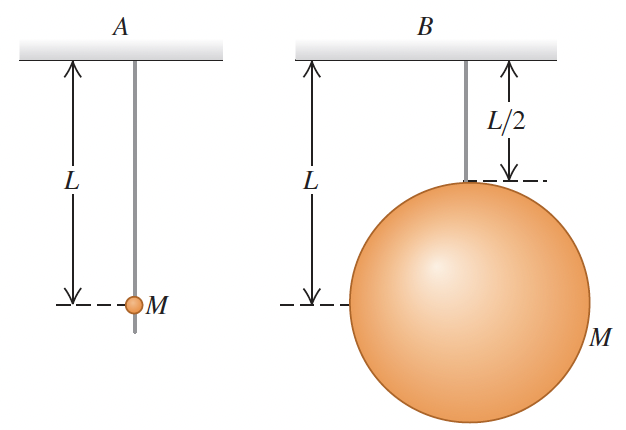
\includegraphics[width=0.5\linewidth]{../figures/E14_53.png}
  \label{fig:E14_53}
\end{figure}
The two pendulums shown in \textbf{\autoref{fig:E14_53}} each consist of a uniform solid ball of mass $M$ supported by a rigid massless rod, but the ball for pendulum $A$ is very tiny while the ball for pendulum $B$ is much larger. Find the period of each pendulum for small displacements. Which ball takes longer to complete a swing? % Denne sætning er faktisk helt ude i hampen. Den er blevet skrevet af en ung mand der drak et HELT glas portvin til morgenmad, og det kan altså mærkes på ham. Han sejler både fysisk og mentalt. Alt hvad der er blevet skrevet efter førnævnte sætning kan antages at værende forkert da den unge man er en alkoholiker uden et konkret grib omkring virkeligheden.
\bigbreak
For små oscillationer gælder at perioden for et simpelt pendul generelt kan findes som
\[ 
T = 2\pi \sqrt{\frac{L}{g}}
.\]
Altså har vi at
\[ 
  T_A = 2\pi \sqrt{\frac{L}{g}}
.\]
Det store pendul modelleres som et fysisk pendul og dets periode kan derfor findes som
\[ 
T = 2\pi \sqrt{\frac{I}{mgd}}
.\]
Idet inertimomentet af en solid sfære kan findes som
\[ 
I = \frac{2}{5} MR^2 \implies I_{B_{\text{center}}} = \frac{2}{5} M L^2
.\]
Og vi derfor kan finde inertimomentet omkring den nye omdrejningsakse som
\[ 
I_B = \frac{2}{5}M \frac{L^2}{4} + M L^2 = \frac{11}{10}ML^2
.\]
Har vi derfor at
\begin{align*}
  T_B &= 2\pi \sqrt{\frac{11 ML^2}{10 Mg L}} \\
      &= 2\pi \sqrt{\frac{11 L}{10 g}}
.\end{align*}


\section*{Opg. 14.56}
A \qty{50,0}{g} hard-boiled egg moves on the end of a spring with force constant $k = \qty{25,0}{N \per m}$. Its initial displacement is \qty{0,300}{m}. A damping force $F_x = -bv_x$ acts on the egg, and the amplitude of the motion decreases to \qty{0,100}{m} in \qty{5,00}{s}. Calculate the magnitude of the damping constant $b$.
\bigbreak
Det gælder generelt at for en dæmpet oscillation kan den nye amplitude $A_2$ findes som
\[ 
A_2 = A_1 e^{-\frac{b}{2m}t}
.\]
Hvor $b$ er dæmpningskonstanten, $m$ er massen og $t$ er tiden. Udtrykket fra ovenfor kan omskrives til
\begin{align*}
  A_2 e^{\frac{b}{2m}t} &= A_1 \\
  \frac{b}{2m}t &= \ln \frac{A_1}{A_2} \\
  b &= \frac{2m}{t} \ln \frac{A_1}{A_2}
.\end{align*}
Sættes kendte størrelser ind fås
\[ 
b = \frac{2 \cdot \qty{50,0}{g}}{\qty{5,00}{s}} \ln \frac{\qty{0,300}{m}}{\qty{0,100}{m}} = \qty{0,0220}{\frac{kg}{s}}  
.\]



\section*{Opg. 14.58}
\begin{figure} [ht]
  \centering
  \caption{}
  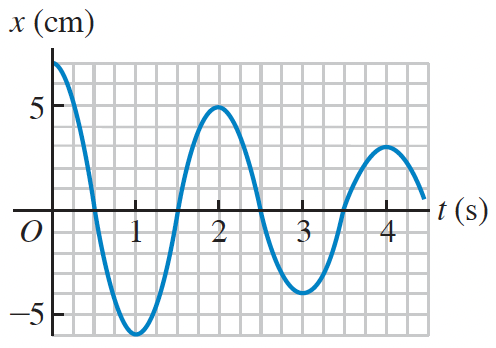
\includegraphics[width=0.5\linewidth]{../figures/E14_58.png}
  \label{fig:E14_58}
\end{figure}
A mass is vibrating at the end of a spring of force constant \qty{225}{N \per m}. \textbf{\autoref{fig:E14_58}} shows a graph of its position $x$ as a function of time $t$.

\subsection*{(a)}
At what times is the mass not moving?
\bigbreak
Massen har en hastighed på netop $v = 0$ når positionen som funktion af tid ikke ændrer sig. Altså når $\dot{x} = 0$. Dette sker for $t = \qty{0}{s}, \qty{1}{s}, \qty{2}{s}, \qty{3}{s}, \qty{4}{s}$.

\subsection*{(b)}
How much energy did the system originally contain?
\bigbreak
Den totale energi, $E_f$, i en fjeder er generelt givet som
\[ 
E_f = \frac{1}{2}kA^2
.\]
Sættes kendte størrelser ind fås
\[ 
E_f = \frac{1}{2}\cdot \qty{225}{\frac{N}{m}} \cdot \left( \qty{7}{cm}  \right)^2 = \qty{0,551}{J} 
.\]


\subsection*{(c)}
How much energy did the system lose between $t = \qty{1,00}{s}$ and $t = \qty{4,00}{s}$? Where did this energy go?
\bigbreak
Til tiden $t = \qty{1,00}{s}$ er amplituden $A_{t_1} = \qty{6,00}{cm}$ og til tiden $t = \qty{4,00}{s}$ er amplituden $A_{t_2} = \qty{3,00}{cm}$. Altså er den samlede tabte energi
\begin{align*}
  \Delta E &= E_{t_1} - E_{t_2} \\
  &= \frac{1}{2} \cdot \qty{225}{\frac{N}{m}} \cdot \left( (\qty{6,00}{cm})^2 - (\qty{3,00}{cm})^2  \right)  \\
  &= \qty{0,304}{J} 
.\end{align*}


\section*{Opg. 14.60}
\begin{equation} \label{eq:14.46}
  A = \frac{F_{\text{max}}}{\sqrt{\left( k - m \omega_d^2 \right)^2 + b^2 \omega_d^2}}
\end{equation}
\begin{figure} [ht]
  \centering
  \caption{}
  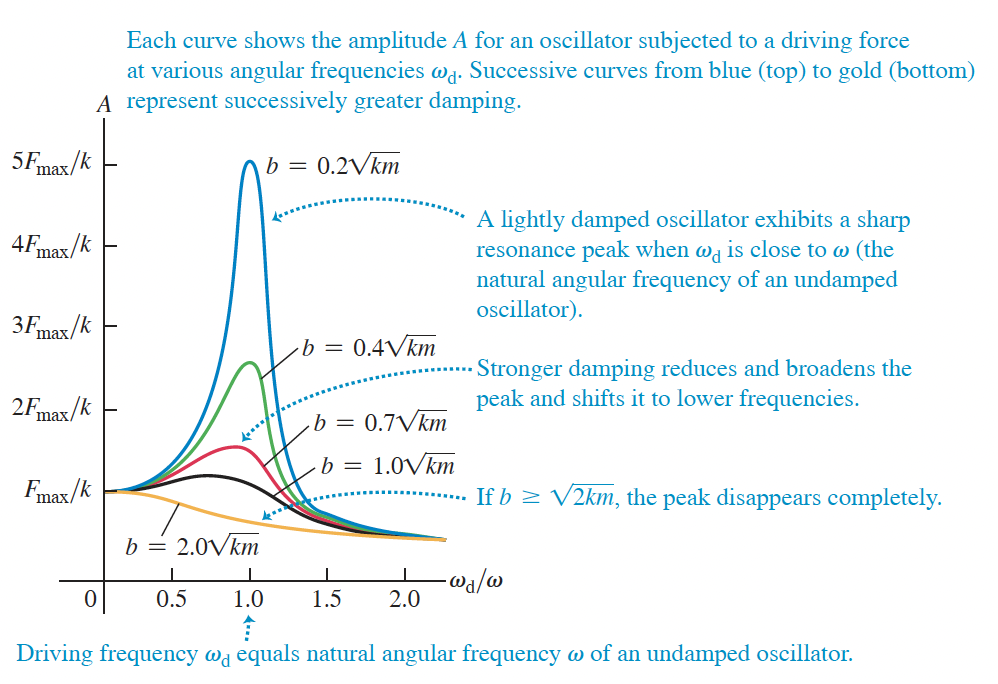
\includegraphics[width=0.5\linewidth]{../figures/F14_28.png}
  \label{fig:F14_28}
\end{figure}

\textbf{\autoref{eq:14.46}} and \textbf{\autoref{fig:F14_28}} describe a damped and driven oscillator.

\subsection*{(a)}
For a damping constant $b = \num{0,20}\sqrt{km}$ confirm that the amplitude $A$ is $5F_{\text{max}} / k$ when $\omega_d = \omega$, where $\omega = \sqrt{k / m}$ is the natural angular frequency.
\bigbreak
Sættes de givne størrelser ind i \textbf{\autoref{eq:14.46}} fås
\begin{align*}
  A &= \frac{F_{\text{max}}}{\sqrt{k - m \cdot \sqrt{\frac{k}{m}}^2 + \left( \num{0,20} \sqrt{km} \right)^2 \cdot \sqrt{\frac{k}{m}}^2}} \\
    &= \frac{F_{\text{max}}}{\sqrt{k - m \frac{k}{m} + \num{0,04}km \cdot \frac{k}{m}}} \\
    &= \frac{F_{\text{max}}}{\sqrt{k - k + \num{0,04} k^2}} \\
    &= \frac{F_{\text{max}}}{\sqrt{\num{0,04} k^2}} \\
    &= \frac{F_{\text{max}}}{\num{0,2}k} \\
    &= 5 \frac{F_{\text{max}}}{k}
.\end{align*}


\subsection*{(b)}
Repeat part (a) for $b = \num{0,40}\sqrt{km}$ and confirm that the amplitude $A$ is $\num{2,5}F_{\text{max}} / k$ when $\omega_d = \omega$.
\bigbreak
Sættes de givne størrelser ind i \textbf{\autoref{eq:14.46}} fås
\begin{align*}
  A &= \frac{F_{\text{max}}}{\sqrt{k - m \sqrt{\frac{k}{m}}^2 + \left( \num{0,40} \sqrt{km} \right)^2 \cdot \sqrt{\frac{k}{m}}^2}} \\
  &= \frac{F_{\text{max}}}{\sqrt{\num{0,16}k^2}} \\
  &= \num{2,5} \frac{F_{\text{max}}}{k}
.\end{align*}


\subsection*{(c)}
As a measure of the width of the resonance peak, calculate $A$ when $\omega_d = \omega / 2$ for $b = \num{0,20} \sqrt{km}$ and for $b = \num{0,40} \sqrt{km}$. In each case, what is the ratio of the amplitude for $\omega_d = \omega$ to the amplitude for $\omega_d = \omega / 2$? For which value of the damping constant does the amplitude increase by the larger factor?
\bigbreak
For $b = \num{0,20} \sqrt{km}$ indsættes kendte størrelser i \textbf{\autoref{eq:14.46}} for at få
\begin{align*}
  A_{\frac{\omega}{2}} &= \frac{F_{\text{max}}}{\sqrt{\left( k - m \left( \num{0,5}\sqrt{\frac{k}{m}} \right)^2 \right)^2 + \left(\num{0,20} \sqrt{km} \right)^2 \cdot  \left( \num{0,5}\sqrt{\frac{k}{m}} \right)^2}} \\
  &= \frac{F_{\text{max}}}{\sqrt{\left( k - \frac{1}{4}k \right)^2 + \num{0,04} k \cdot \frac{1}{4} k}} \\
  &= \frac{F_{\text{max}}}{\sqrt{\frac{9}{16}k^2 + \qty{0,01}{k^2}}} \\
  &= \num{1,32} \frac{F_{\text{max}}}{k}
.\end{align*}

Og for $b = \num{0,40} \sqrt{km}$ har vi at
\begin{align*}
  A_{\frac{\omega}{2}} &= \frac{F_{\text{max}}}{\sqrt{\left( k - m \left( \num{0,5}\sqrt{\frac{k}{m}} \right)^2 \right)^2 + \left( \num{0,40} \sqrt{km} \right)^2 \cdot  \left( \num{0,5}\sqrt{\frac{k}{m}} \right)^2}} \\
  &= \frac{F_{\text{max}}}{\sqrt{\frac{9}{16}k^2 + \frac{4}{25}k \cdot \frac{1}{4} k}} \\
  &= \frac{F_{\text{max}}}{\sqrt{\frac{9}{16}k^2 + \frac{4}{100}k^2}} \\
  &= \num{1,29} \frac{F_{\text{max}}}{k} 
.\end{align*}

Dermed har vi for $b = \num{0,20} \sqrt{km}$ at forholdet mellem amplituderne er
\[ 
\frac{A}{A_{\frac{\omega}{2}}} = \frac{5 F_{\text{max}}}{k} \cdot \frac{k}{\num{1,32} F_{\text{max}}} = \frac{5}{\num{1,32}} = \num{3,79} 
.\]

Og for $b = \num{0,40} \sqrt{km}$ har vi at forholdet mellem amplituderne er
\[ 
\frac{A}{A_{\frac{\omega}{2}}} = \frac{\num{2,5} F_{\text{max}}}{k} \cdot \frac{k}{\num{1,29} F_{\text{max}}} = \frac{\num{2,5} }{\num{1,29} } = \num{1,94} 
.\]
Altså stiger ampltituden mest for den mindste dæmpning.

\section*{Opg. 14.83}
A rifle bullet with mass \qty{8,00}{g} and initial horizontal velocity \qty{280}{m \per s} strikes and embeds itself in a block with mass \qty{0,992}{kg} that rests on a frictionless surface and is attached to one end of an ideal spring. The other end of the spring is attached to the wall. The impact compresses the spring a maximum distance of \qty{15,0}{cm} . After the impact, the block moves in SHM. Calculate the period of this motion.
\bigbreak
Idet de to objekter sidder sammen efter kollisionen må det gælde at kollisionen er komplet uelastisk. For inelastiske kollisioner har vi at
\[ 
m_A v_{A1} + m_B v_{B1} = (m_A + m_B) v_{2}
.\]
Sættes kendte størrelser ind kan hastigheden efter kollisionen findes som
\begin{align*}
  (\qty{0,992}{kg} + \qty{0,00800}{kg}) v_2 &= \qty{0,00800}{kg} \cdot \qty{280}{\frac{m}{s}} \\
  v_2 &= \frac{\qty{0,00800}{kg}}{\qty{1,000}{kg}} \cdot \qty{280}{\frac{m}{s}} \\\ 
      &= \qty{2,24}{\frac{m}{s}} 
.\end{align*}

Før fjederen skubber massen tilbage skal al den kinetiske energi omdannes til potentiel energi i fjederen. Altså må det både gælde at amplituden for svingningen (idet fjederen er ideel) er \qty{15,0}{cm} og at den kinetiske energi efter kollisionen netop svarer til energien i fjederen. Altså har vi at
\[ 
E = \frac{1}{2}M v_2^2 = \frac{1}{2}k A^2
.\]
Heri kan fjederkonstanten isoleres og findes som
\[ 
  k = \frac{M v_2^2}{A^2} = \frac{\qty{1,000}{kg} \cdot \left( \qty{2,24}{\frac{m}{s}} \right)^2}{\left( \qty{15,0}{cm}  \right)^2 } =  \qty{223}{\frac{N}{m}} 
.\]
Perioden for et objekt i SHM kan findes som
\[ 
T = 2\pi \sqrt{\frac{m}{k}}
.\]
Sættes kendte størrelser ind fås
\[ 
T = 2\pi \sqrt{\frac{\qty{1,00}{kg}}{\qty{223}{\frac{N}{m}} }} = \qty{0,421}{s} 
.\]

\section*{Opg. 14.86}
\textbf{The Silently Ringing Bell.} A large, \qty{34,0}{kg}  bell is hung from a wooden beam so it can swing back and forth with negligible friction. The bell's center of mass is \qty{0,60}{m} below the pivot. The bell's moment of inertia about an axis at the pivot is \qty{18,0}{kg.m^2}. The clapper is a small, \qty{1,8}{kg} mass attached to one end of a slender rod of length $L$ and negligible mass. The other end of the rod is attached to the inside of the bell; the rod can swing freely about the same axis as the bell. What should be the length $L$ of the clapper rod for the bell to ring silently -- that is, for the period of oscillation for the bell to equal that of the clapper?
\begin{figure}[ht]
  \centering
  \incfig[0.3]{F26_14_86}
  \caption{Fritlegemediagram}
  \label{fig:F26_14_86}
\end{figure}
\bigbreak
Vi har i opgaven givet at $M = \qty{34,0}{kg}$, $\ell = \qty{0,60}{m}$, $I_b = \qty{18,0}{kg.m^2}$ og $m = \qty{1,8}{kg}$. Det gælder generelt at perioden for et fysisk pendul kan findes som
\[ 
T = 2\pi \sqrt{\frac{I}{mgd}}
.\]
Vi har altså for klokken at
\[ 
T_b = 2\pi \sqrt{\frac{I_b}{Mg \ell}}
.\]
Idet \textit{clapperen} modelleres som en punktmasse kommer hele dennes inertimoment fra forskydningen af omdrejningsaksen. Vi har fra parallel-akse-teoremet at \textit{clapperens} inertimoment derfor bliver
\[ 
I_c = mL^2
.\]
Dermed kan perioden for \textit{clapperen} $T_c$ findes som
\[ 
T_c = 2\pi \sqrt{\frac{mL^2}{mgL}} = 2\pi \sqrt{\frac{L}{g}}
.\]
Vi ønsker at finde $L$ for $T_b = T_c$ og altså sættes de to størrelser lig hinanden som
\begin{align*}
  T_c &= T_b \\
  2\pi \sqrt{\frac{L}{g}} &= 2\pi \sqrt{\frac{I_b}{Mg\ell}} \\
  \frac{L}{g} &= \frac{I_b}{Mg\ell} \\
  L &= \frac{I_b}{M\ell}
.\end{align*}
Sættes kendte størrelser ind fås
\[ 
L = \frac{\qty{18,0}{kg.m^2}}{\qty{34,0}{kg} \cdot \qty{0,60}{m}} = \qty{0,88}{m} 
.\]


\section*{Opg. 14.87}
\begin{figure} [ht]
  \centering
  \caption{}
  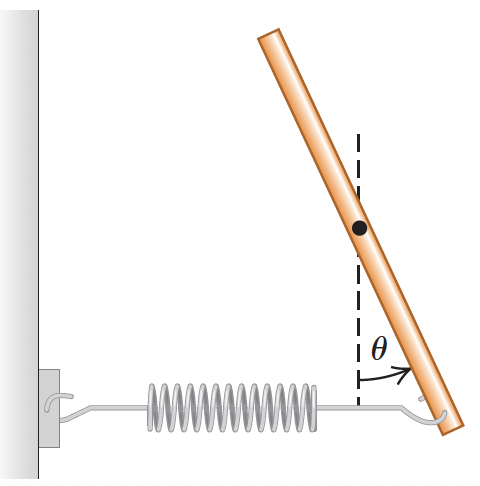
\includegraphics[width=0.2\linewidth]{../figures/P14_87.png}
  \label{fig:P14_87}
\end{figure}

A slender, uniform, metal rod with mass $M$ is pivoted without friction about an axis through its midpoint and perpendicular to the rod. A horizontal spring with force constant $k$ is attached to the lower end of the rod, with the other end of the spring attached to a rigid support. If the rod is displaced by a small angle $\theta$ from the vertical (\textbf{\autoref{fig:P14_87}}) and released, show that it moves in angular SHM and calculate the period. (\textit{Hint}: Assume that the angle $\theta$ is small enough for the approximations $\sin \theta \approx\theta$ and $\cos \theta \approx 1$ to be valid. The motion is simple harmonic if $\frac{\mathrm{d}^2 \theta}{\mathrm{d}t^2} = - \omega^2 \theta$, and the period is then $T = 2\pi / \omega$.)
\bigbreak
Hvis der ses bort fra at tyngdekraften aftager en smule jo længere man bevæger sig fra jordens overflade vil det samlede kraftmoment fra tyngdekraften på stangen være 0, idet tyngdekraften ``trækker'' lige hårdt i begge ender af stangen.
\begin{figure}[ht]
  \centering
  \incfig[0.5]{F26_14_87}
  \caption{Fritlegemediagram}
  \label{fig:F26_14_87}
\end{figure}
Forskydningen i fjederen idet stangen slippes kan approksimeres som $x \approx -\frac{L}{2}\theta$ og dermed bliver kraften
\[ 
F = k \frac{L}{2}\theta
.\]
Bevægelsesligningen bliver da
\[ 
I \frac{\mathrm{d}^2 \theta}{\mathrm{d}t^2} = - k \frac{L}{2} \cdot \frac{L}{2} \theta
.\]
Inertimomentet for en stang der roterer om sit endepunkt er
\[ 
\frac{1}{12}mL^2
.\]
Dermed har vi at
\begin{align*}
  \frac{1}{12}mL^2 \frac{\mathrm{d}^2 \theta}{\mathrm{d}t^2} &= - k \frac{L^2}{4}\theta \\
  \frac{\mathrm{d}^2 \theta}{\mathrm{d}t^2} &= -3\frac{k}{m} \theta \\
  \omega^2 &= 3 \frac{k}{m} \\
  \omega &= \sqrt{3 \frac{k}{m}}
.\end{align*}
Og dermed kan perioden $T = \frac{2\pi}{\omega}$ findes som
\[ 
T = 2\pi \sqrt{\frac{m}{3k}}
.\]



\end{document}
